\chapter{Appendix - Math Prerequisites}

\section{GMM Log Probability Value}
\label{appendix:gmm_log_prob}
For a two-dimensional \ac{GMM} $g \sim GMM(\mu, \Sigma, \pi, \rho)$ with mean vector $\mu$, variance matrix $\Sigma$, mode importance vector $\pi$ and Pearson's correlation coefficients $\rho$ the probability at $(x, y)$ can be computed as:\footnote{\href{https://de.wikipedia.org/wiki/Mehrdimensionale_Normalverteilung}{Wikipedia - Multivariate Normal Distribution}}.

\begin{align}
f_m(x, y | \mu, \sigma, \rho) 
&= \frac{1}{2 \pi \sqrt{\det \Sigma}} \exp \left(- \frac{1}{2} (\boldsymbol{x} - \boldsymbol{\mu})^T \Sigma (\boldsymbol{x} - \boldsymbol{\mu}) \right) \\
&= {\frac{\sqrt{1- \rho^2}}{2 \pi \sigma_x \sigma_y} 
\exp - \frac{1}{2 (1 - \rho^2)}} \left( \frac{( x - \mu _x)^2}{\sigma_x^2} +
\frac {(y - \mu_y)^2}{\sigma_y^2}-{\frac {2\rho (x - \mu_x)(y - \mu_y)}
{\sigma_x \sigma_y}} \right)	
\end{align}

The Pearson coefficient is the covariance for two normalized random variables $X$ and $Y$, in their normalized form $\tilde{X} = (X - \mu_x)/\sigma_x$ and $\tilde{Y} = (Y - \mu_y) / \sigma_y$. Using the law of linear transformations of covariances we get:\footnote{\href{https://en.wikipedia.org/wiki/Pearson_correlation_coefficient}{Wikipedia - Pearson correlation coefficient}} 

\begin{equation}
Cov(\tilde{X}, \tilde{Y}) = \frac{1}{\sigma_x \sigma_y} Cov(X, Y) = \rho_{X, Y}
\end{equation}

The expected value over all modes $m \in [0, M]$ super-imposes the \ac{PDF} for the bi-variate Gaussian distributions, weighting each one by its importance $\pi_m$:

\begin{equation}
\mathbb{E}_{GMM}[x, y] = \sum_{m=0}^M \pi_m \cdot f_m(x, y) =  \sum_{m=0}^M \exp \left( \log \pi_m + \log f_m(x, y) \right)	
\end{equation}


%\begin{figure}[ht!]
%\begin{center}
%\begin{tikzpicture}[node distance=1cm, auto,]
%
%\node[rectangle, rounded corners, draw=black, very thick, text width=8.5em,
%      minimum height=2em, text centered](intermediate) {Pedestrian States\\$\muped[j]_t, \sigmaped[j]_t$};
%\node[rectangle, rounded corners, draw=black, very thick, text width=8.5em,
%      minimum height=2em, text centered, below=0.5cm of intermediate](robot) {Robot state\\$\x_t$};
%
%\node[above=of intermediate] (dummy) {};
%\node[right=of dummy] (t) {Particle simulation()}
%   edge[<-, bend left=45] (robot.east)
%   edge[<-, bend left=45] (intermediate.east); 
%\node[left=of dummy] (g) {Accumulation()}
%   edge[->, bend right=45] (intermediate.west)
%   edge[<-, bend left=45] (t)
%   edge[<-, bend left=50] (t)
%   edge[<-, bend left=40] (t);
%\end{tikzpicture}
%\end{center}
%\caption{...}
%\label{fig:particle_simulation}
%\end{figure}


%\chapter{Problem Definition}
%\label{chp:problemDefinition}
%In this work, we are interested in deriving a trajectory planning algorithm based on the Trajectron behavioral prediction model \cite{Ivanovic18}. The Trajectron combines elements of variational deep generative models (\ac{VAE}), recurrent sequence models (\ac{LSTM}) and dynamic spatio-temporal graphical structures to predict the possible movements, i.e. velocity distributions, of each agent in a scene, given their state trajectories. 
%
%\begin{figure}[h]
%\centering
%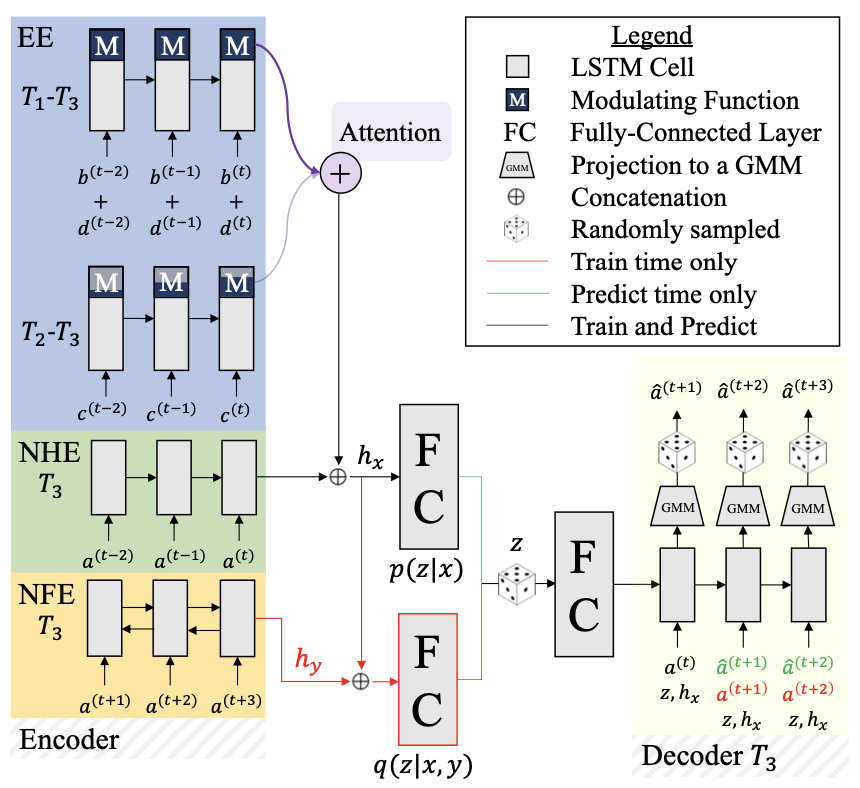
\includegraphics[width=0.5\textwidth]{images/trajectron.png}
%\caption{Trajectron model architecture  \cite{Ivanovic18}}
%\label{fig:trajectron_architecture}
%\end{figure}
%
%The architecture of Trajectron is shown in Fig. \ref{fig:trajectron_architecture}. First the history of each agent (node) is as well as their relations between each other (edges) are encoded, added and transformed to a discrete latent space $z$. By random sampling from $z$ the future velocity distributions are predicted iteratively. In order to approximate a multi-modal, general distribution for every time-step a \ac{GMM} is used. While unrolling the For each $0 < t < T$ in the prediction horizon a sample is drawn from the previously predicted distribution and inputted in the next \ac{LSTM} cell. Therefore, the velocity distribution of each agent in the scene for $t > 1$ is modelled as a nested \ac{GMM} distribution (the velocity distribution at $t = 0$ is a \ac{GMM}). 
%\newline
%In general a planning algorithm that determines a trajectory that is risk-aware of colliding with another agent based on the behavior predictions of the Trajectron model has to deal with multi-modal and time-evolving risk efficiently. Since each distribution depends on the full state history, not on the last state only, the transitions are a \ac{POMDP} (given that not the full history is part of the state vector). For simplicity we assume the ego's dynamics to be known and deterministic. Formally speaking we want to optimize a given cost function $J(x(t), u(t))$ while being constrained by some collision risk threshold $R_{max}$: 
%
%\begin{equation}
%\begin{aligned}
%\min_{x(t), u(t)} \quad & J(x(t), u(t)) = \sum_{k = 0}^{N-1} l(x_k, u_k) + l_f(x_N) \\
%\textrm{subject to} \quad & x_{k + 1} = f_{ego}(x_k, u_k) \\
%    &x_0 = x(0) \\
%    &x_N = x_{goal} \\
%    &\sum_{k = 0}^N r(x_k, u_k) \leq R_{max} \\
%\end{aligned}
%\end{equation}
%
%
%\chapter{Related Approaches}
%\label{chp:AppendixRelatedApproaches}
%
%\begin{itemize}
%    \item Chance-Constrained Model Predictive Control \cite{Lew2019}, \cite{Ono2015CCMPC}, \cite{Ono2012}, \cite{Blackmore2012}, \cite{chow2015DTRC}, \cite{ono2008}: CCMPC minimizes the cost function $J(x(t), u(t))$ with respect to a point-wise risk allocation constraint. Therefore the solution is guaranteed to be first-order and locally optimal (comp. \cite{bonalli2019}) and to fulfill the risk constraint, instead of deriving some trade-off between risk and cost (when the risk would be part of the cost function). However the constrained risk distribution is neither convex nor linear, therefore it cannot be used directly in a constraint (efficiently), but has to be reformulated as following (re-approximate in every step, SQP). To reformulate these constraints the distribution has to be remodelled in "analytically" expressible distributions: 
%    
%    \begin{itemize}
%        \item Mean-variance analysis ("ellipsoidal" overlapping) \cite{herzog2006}, \cite{hewing2018}, \cite{Lew2019} (when $y ~ N(\mu, \Sigma)$ and $\chi = $ quantile of chi-squared distribution): 
%        
%        $$Pr(||x - y||_2 \geq r) \geq \rho_{max}$$ $$||x-\mu||_2 + \lambda_{max}(\sigma) * \chi(\rho_{max}) \geq r$$
%        
%        \item Cone Constraint (\cite{calafiore2006}, \cite{Lew2019})
%    \end{itemize}
%    
%    Following \cite{ono2008} the risk allocation and the control sequence with tightened constrained can be divided in two steps (iterative risk allocation), in order to be less conservative in estimating the real risk and more computationally efficient.
%    
%    \item Belief Space Planning using Sequential Action Control \cite{ansari2017}, \cite{nishimura2019}: Given some nominal trajectory (e.g. just going straight from start to goal position) find the optimal perturbation for optimizing control objective (J = Tracking + Control + RBF for risk, entropy risk, risk-awareness of ego is controlled by $\sigma$-factor in risk-related control objective) by forward simulation and backward derivation of Hamiltonian.
%    
%    \item Chance-Constrained Rapidly-Exploring Random Trees \cite{Luders2011}, \cite{Luders2010}, \cite{Luders2013}, \cite{Aoude2013}: Under the assumption of linear Gaussian systems RRT can be used for chance-constrained trajectory optimization in continuous space by propagating both the mean and the variance of a state. CC-RRTstar guarantees asymptotic optimality, while a particle based approach can be used for non-linear system dynamics. As shown in \cite{Aoude2013} this approach can be used for dynamic and uncertain obstacles such as pedestrians. While not being applicable to "proper" real-time learned sampling distributions can be used to speed up convergence \cite{Ichter2017}.
%    
%    \begin{figure}[H]
%    \centering
%    \includegraphics[width=0.4\textwidth]{images/rrtcc_loop.png}
%    \includegraphics[width=0.4\textwidth]{images/rrtcc_expansion.png}
%    \caption{Chance-constrained RRT algorithm \cite{Luders2013}}
%    \label{fig:rrtcc}
%    \end{figure}
%  
%    \item Multi-Policy Decision-Making \cite{Galceran2017}: Based on a set of (pre-computed) policies first match the observed behavior of each agent to some policy (Baysian changepoint detection), then sample from policy in order to obtain high-likelihood action for each agent. Afterwards forward simulate all assigned policies and execute the policy with maximum expected reward value. 
%    
%    \begin{figure}[H]
%    \centering
%    \includegraphics[width=0.5\textwidth]{images/mulitpolicy_policy_section.png}
%    \caption{Policy selection algorithm \cite{Galceran2017}}
%    \label{fig:mulitpolicy_policy_section}
%    \end{figure}
%    
%    \item Chance-Constrained Dynamic Programming \cite{Ono2015DP}, \cite{chow2015}
%    
%    \item \ac{POMDP} solver (e.g. POMDP-lite \cite{Chen2016} or DESPOT-alpha \cite{Garg2019}): In general the state transitions in the Trajectron model are \ac{POMDP}s. When discretizing states (continuou => particle filter) and actions a policy can be determined that maximizes some human-engineered utility function, given random state transitions as defined by the Trajectron model. Although computationally very expensive, especially it scales badly with increasing space resolution, the solution in theory should be (globally) optimal. Similarly online belief state planning methods such as Monte Carlo tree search (e.g. POMCP \cite{silver2010}), Lookahead with approximate value function, etc. might be used (maybe based on some offline-computed utility function). However the problem's structure is not used that could safe computational expenses. 
%    
%    \item Deep Reinforcement Learning \cite{Chen2017}, \cite{Everett2018}: Socially aware reinforcement learning approach mapping directly from ego's and other agent's joint state to a trajectory: 
%    
%    \begin{align*}
%        s &= \begin{bmatrix} s_{ego} & s_{o} \end{bmatrix} \\
%        s_{ego} &= \begin{bmatrix} d_g& v_{pref} & v_x & v_y & \psi & r  \end{bmatrix} \\
%        s_o &= \begin{bmatrix} \title{p}_x & \title{p}_y & \title{v}_x & \title{v}_y & \tilde{r} & \tilde{d}_a & \title{\phi} & \tilde{b}_{on} \end{bmatrix}
%    \end{align*}
%    
%    while the reward function is a sum of human-engineered encoded social norms (e.g. right-hand rule). 
%    
%    \begin{figure}[H]
%    \centering
%    \includegraphics[width=0.5\textwidth]{images/DRL_socially_aware.png}
%    \caption{DRL update rule \cite{Everett2018}}
%    \label{fig:DRL_socially_aware}
%    \end{figure}
%    
%    \item Safe-Interval Planning \cite{Phillips2011}: Efficient AStar graph search for dynamic obstacles using time-intervals instead of single time-steps for planning, in order to avoid the increase in the dimensionality of the planning problem with increasing time horizon (safe intervals = time-intervals without collision). SIPP provides the same optimality and completeness guarantees as planning with time as an additional dimension (time-steps). For every grid cell the sequence of safe and collision intervals is defined based on a risk-threshold (i.e. point-wise risk allocation). 
%    
%    \item Inverse Reinforcement Learning \cite{Tschiatschek2019}: In order to shrink the search space for finding a trajectory inverse reinforcement learning can be used based on the offline computation of "good" trajectories (e.g. human demonstration, brute-force, DESPOT, etc.) for some scenarios. Thereby the reward function can be built, which basically can be used as a single, static cost-map which can be used by "standard" path planning algorithms such as Dijkstra to find an optimal trajectory. As shown in \cite{Tschiatschek2019} IRL can be used to both match the teacher’s demonstrated behavior but also takes its constraints, such as physical constraints of the ego dynamics or point-wise risk constraints. However a lot of optimal trajectories still are required for training. Compared to mapping from the observations to the policy directly using IRL is more tractable, since the resulting cost map might be interpretable. 
%    
%    \item Adaptive Dimensionality \cite{Vemula2016}
%    
%    \item Signal Temporal Logic \cite{Sadigh2016}
%    
%    \item Optimal Reciprocal Collision Avoidance \cite{Ma2018} \cite{Berg2011} \cite{Hennes2012} \cite{Luo2018}: Local collision avoidance algorithm modeling the pedestrians as velocity obstacles with deterministic (just one or a set of) velocity. To determine the velocity of every agent in the scene for every pair of agents a set $VO_{A|B}^\tau$ (the velocity obstacle for $A$ induced by $B$ for time window $\tau$) is constructed. Using LP the minimal velocity adaption for every agent is determined so that no pair of velocities is in some velocity obstacle set, assuming that all agents follow the same strategy (!). In \cite{Luo2018} ORCA is adapted to model pedestrian movement by e.g. introducing a notion of patience and to deal with non-holonomic dynamics (P-ORCA). Using Hyp-DESPOT in every time-step the belief of the pedestrians intentions is updated (actions = [ACCELERATE, DE- CELERATE, or MAINTAIN] and some human-engineered reward function trading collision and speed of the agent), which is used for a path update (Hybrid Astar) and velocity updates (P-ORCA).  
%
%\end{itemize}
%
%There are several categories from which the properties of planning approaches can be evaluated: 
%
%\begin{itemize}
%    \item Optimality: trajectory cost vs minimal possible (optimal) cost
%    \begin{itemize}
%        \item globally: $J(x(t), u(t)) = J^*(x(t), u(t)) \forall t$
%        \item locally: $J(x(t), u(t)) \approx J^*(x(t), u(t)) \forall x(t) + \epsilon, u(t) + \epsilon $
%        \item not at all
%    \end{itemize}
%    
%    \item Risk-Awareness: Point-wise constraints are easier to fulfill since each state can be regarded individually, however it assumes independence between the states, which is clearly not given due to the dynamical constraints of the ego. As shown in \cite{JansonSP15} both the additive and multiplicative formulation do not scale with increasing planning horizon, since the accumulated risk converges to infinity. Also the using point-wise constraint often is a very conservative choice, as it does not allow to take more risk at some point to be more efficient or to save risk somewhere else. 
%    \begin{itemize}
%        \item trajectory-wise: $\sum_{k = 0}^N r(x_k, u_k) \leq R_{max}$
%        \item point-wise: $r(x_k, u_k) \leq R_{max} \forall k$
%    \end{itemize}
%
%    \item Computational Feasibility:  
%    \begin{itemize}
%        \item real-time planning
%        \item online policy/trajectory correction (e.g. using perturbation) 
%        \item not real-time applicable
%    \end{itemize}
%    
%    \item Explainability/Tractability \& Guarantees: When the result of the planning algorithm is not tractable it is very hard (or even impossible) to give theoretical guarantees with respect to safety constraints. Therefore for these approaches an additional step, determining the empirical risk of collision using Monte Carlo simulations, is necessary, at the cost of additional run-time.  
%\end{itemize}
%
%\begin{center}
%\begin{tabular}{c||p{2cm}|p{1cm}|p{2cm}|p{1cm}|p{1cm}|p{1cm}|p{1cm}|p{1cm}}
%    Method & 
%    \rotatebox[origin=c]{90}{Space ?} &  \rotatebox[origin=c]{90}{Risk-Awareness ?} & 
%    \rotatebox[origin=c]{90}{PPDF Model ?} & 
%    \rotatebox[origin=c]{90}{Risk as cost ?} &
%    \rotatebox[origin=c]{90}{Optimality ?} &
%    \rotatebox[origin=c]{90}{Parametrization ?} &
%    \rotatebox[origin=c]{90}{Interactive ?} &
%    \rotatebox[origin=c]{90}{Tractability ?} \\
%    \hline\hline
%    
%    CCMPC & continuous & point-wise & approximate (uni-Gaussians) & no & locally & sparse & no & yes \\
%    \hline
%    SIPP & discrete & point-wise & accurate (sampled GMM) & no & globally & sparse & no & yes \\
%    \hline
%    DRL & continuous & none & none & no & none & much & yes & no \\
%    \hline
%    PORCA & continuous & none & none & none & none & much & yes & no \\
%    \hline
%    SACBP & continuous & yes & accurate (sampled traject.) & yes & locally & sparse & no & yes \\
%    \hline
%    POMDP & discrete & yes & accurate & yes & globally & much (state definition) & no & yes \\
%    \hline
%    IRL & discrete & yes & accurate & none & none & much (optimal trajectory) & medium & medium
%    
%\end{tabular}
%\end{center}
%
%
%\chapter{Ideas}
%\label{chp:AppendixIdeas}
%
%\section{Planning Approaches}
%\label{sec:planning_approaches}
%
%
%\section{Approximation Approaches}
%\label{sec:approximation_approaches}
%Over a time horizon t > 1 the Trajectron model predicts by sampling from the previously generated distribution. Therefore the distribution of velocities over multiple time-steps is a nested GMM. While samples from the distribution are accessible by iteratively applying the model and can be easily forward integrated (since position-based information are more straight forward to integrate in most planners) getting the distributions themselves is not straight-forward. However it can be approximated: 
%
%\begin{itemize}
%    \item Sample trajectories from the model, integrate them and approximate the obtained distribution 
%    \begin{itemize}
%        \item \ac{GMM}s basically are proxies for modelling some distribution, therefore for every time-step also a GMM could be used to model the obtained samples to a distribution (how many kernels ? = modes x obstacles or less)
%        \item Each mode (i.e. $z_i$ in latent space of Trajectron) can be sampled from individually and modelled per time-step as 2D Gaussian ($\Sigma_{xy} = 0$ for comp. reasons), which is requires more sample-inefficient but directly gives you a sense of importance of each Gaussians due to the value of the mode in the latent space
%        \item[+] fairly easy and tractable
%        \item[$-$] approximative, no regularity constraints between subsequent time-steps (however I am not sure whether this is desirable ?)
%    \end{itemize}
%    
%    \item Adapting Trajectron model: Problematic about the way the Trajectron model iteratively builds the velocity distributions is not that they are nested but that the nesting is random and therefore not simply tractable. In order to overcome this issue the Trajectron model can be adapted in one of the following ways: 
%    \begin{itemize}
%        \item  only propagate a specific point (e.g. the mean of the most probable mode) to the next \ac{LSTM} cell
%        \item base next time-step on the previous prediction but predict it without sampling from the previous distribution. 
%    \end{itemize}
%    
%    \begin{figure}[h]
%    \centering
%    \includegraphics[width=0.5\textwidth]{images/idaes_simplification.jpeg}
%    \caption{Ideas for Trajectron model simplification}
%    \label{fig:trajectron_simplifaction}
%    \end{figure}
%    
%\end{itemize}
%
%
%\section{Evaluation}
%\label{sec:evaluation}
%For evaluation some underlying distribution for the obstacles/pedestrians is assumed and sampled during testing time. During repeated experiments while the ego always drives the same planned trajectory, the agents sample and execute velocities from their underlying distributions. 
%
%\begin{itemize}
%    \item Monte-Carlo simulations (i.e. use derived policy and simulate N runs while sampling from distribution, comp. \cite{Ono2015}) with the following measures
%    \begin{itemize}
%        \item empirical probability of failure vs risk
%        \item comfort (smooth acceleration, etc.)
%        \item travel-time
%        \item minimal distance to obstacles
%    \end{itemize}
%    
%    \item (eventually) human in the loop comparison (steering wheel)
%\end{itemize}
%
%
%\section{Baseline}
%\label{sec:baseline}
%\begin{itemize}
%    \item Uni-modal velocity distribution by merely taking into account most probable mode into account for the agent's movement prediction in order to show the advantage of multi-modality for the planning algorithm
%    
%    \item Static velocity distribution by merely taking into account the velocity distribution at $t = 0$ in order to show the advantage of longer prediction horizon
%    
%    \item Constant velocity over time (either last velocity or mean of most probable mode) in order to show the advantage of using distributions over deterministic states 
%    
%    \item Kalman velocity and uncertainty propagation using pedestrian integrator dynamical model
%    
%    \item Brute force try and error by using some planning algorithm (e.g. RRT) multiple times while selecting the path with minimum approximate path collision probability (comp. \cite{JansonSP15})
%\end{itemize}
